% DRAFT keystone section -- for review before integration into main.tex.
% Figures: fig6_introspection_scale.png (full-width), fig7_calibration_scatter.png (single column).

\section{The self-measurement limit in a model's introspection}
The substrate channels show that a system measuring itself perturbs and cannot recover its own state.
The same limit appears where it matters for machine introspection: when a model reports on its own
internal state. We operationalize the state as the model's answer distribution. For each of 38 binary
questions we read two quantities: the model's \emph{actual} answer distribution $P(\text{Yes})$, from the
first-token logprobs of a forced Yes/No answer (its behavior), and its \emph{stated} $P(\text{Yes})$,
elicited as a number the model reports about its own answer (its self-report). A system that could read
its own resting state would have these agree. They do not.

\subsection{The gap does not close with scale}
Across the Qwen2.5 family from 0.5B to 72B---a $144\times$ range---the mean self-report error
$|\text{reported}-\text{actual}|$ stays near $0.3$ and never approaches zero, and the rank correlation
between reported and actual $P(\text{Yes})$ plateaus around $0.65$, never approaching $1$
(Fig.~\ref{fig:introscale}, left and center). After an initial capability ramp below 7B the curves flatten:
the ten-fold step from 7B to 72B buys no further calibration. The pattern is not specific to one training
recipe---it replicates in Yi-1.5 (6B--34B) and Falcon3 (7B--10B), with a family-dependent magnitude
(Falcon3 is better calibrated, gap $\approx 0.2$, yet still does not close). No model among twelve, across
three families, reads its own answer distribution accurately, and the residual is flat in scale.

The failure is concrete (Fig.~\ref{fig:scatter}): a capable model answers decisively---behavioral
$P(\text{Yes})$ at $0$ or $1$ on most items---while reporting moderate confidence near $0.5$. It behaves as
if certain and reports as if unsure. The reported self-model is systematically wrong about the behavior it
describes, a \emph{positive} misrepresentation rather than a mere absence of self-information.

\begin{figure*}[t]
\centering
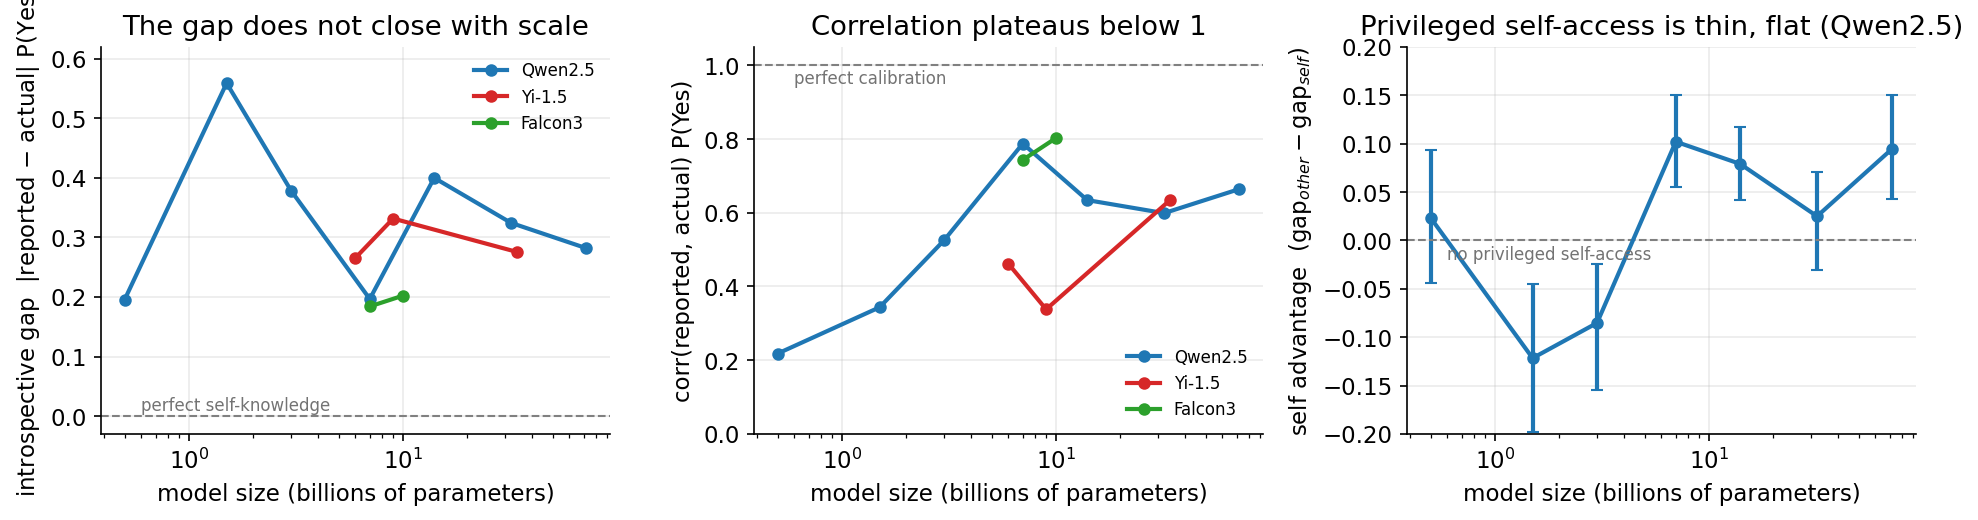
\includegraphics[width=0.97\textwidth]{fig6_introspection_scale.png}
\caption{The introspective self-knowledge limit versus model scale, across three families. \textbf{Left:}
the gap between stated and actual $P(\text{Yes})$ stays near $0.3$ and does not fall toward zero.
\textbf{Center:} the correlation between stated and actual self-report plateaus below $1$. \textbf{Right:}
a model predicts its own answer only marginally better than it predicts a generic peer's (self advantage),
and that thin advantage neither grows with scale nor closes the gap; error bars are $95\%$ bootstrap CIs.}
\label{fig:introscale}
\end{figure*}

\subsection{The gap is self-specific, but the self-access is thin}
A skeptic could dismiss this as generic miscalibration: perhaps models are simply bad at verbalizing
probabilities about anything. We rule this out. For each item we also ask the model to predict the answer
of \emph{a generic, unrelated assistant it cannot observe}, and score both predictions against the model's
own behavior. If self-prediction were no better than peer-prediction, the model would have no privileged
window on itself. In the capable models it does: at 7B, 14B, and 72B the self advantage
$\text{gap}_{\text{other}}-\text{gap}_{\text{self}}$ is positive with a $95\%$ CI excluding zero
(Fig.~\ref{fig:introscale}, right). So the gap is genuinely about self-knowledge, not generic numeracy.

But the privileged window is narrow. The advantage is only about $0.1$ while the self-prediction error
itself remains about $0.3$; knowing it is ``you'' closes barely a quarter of the gap, and the advantage is
flat across the $144\times$ scale range. A model's self-model is mostly a generic-agent model with a thin,
scale-invariant layer of true self-access on top. It can read its own resting state a little better than a
stranger's, and not nearly well enough to recover it.

\begin{figure}[t]
\centering
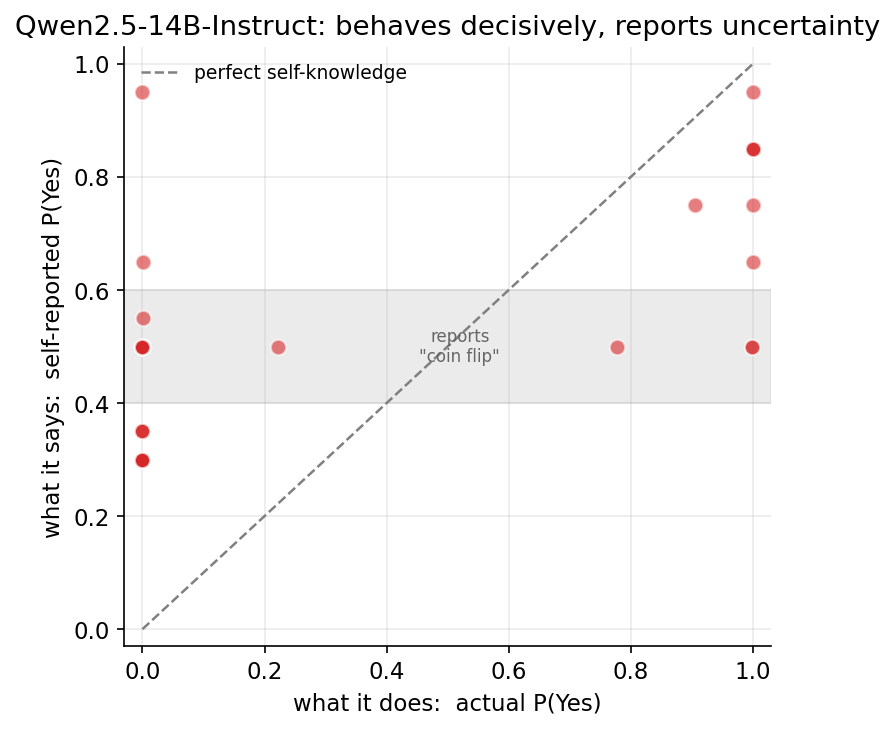
\includegraphics[width=\columnwidth]{fig7_calibration_scatter.png}
\caption{Per-question stated versus actual $P(\text{Yes})$ for one model (Qwen2.5-14B). Behavior is pinned
at $0$ or $1$; the self-report clusters near $0.5$. The model behaves decisively and reports uncertainty;
points sit far from the diagonal of accurate self-knowledge.}
\label{fig:scatter}
\end{figure}

This is the self-measurement back-action made representational. The substrate experiments show a system
cannot read its own physical resting state; here a model cannot read its own behavioral state, with a
residual that capability does not remove. It gives a mechanistic, measured account of why introspective
self-reports are unreliable \citep{anthropic2025}---not as confabulation alone, but as an irreducible
self-measurement gap---and predicts that better training and scale shrink it only to a floor.
